\chapter{Introduction}
\label{chapter:introduction}

	What was/is the purpose of this thesis? Why did we develop these computational simulations? Really, we need a goal!

%In this thesis, a lattice Monte Carlo approach was used to simulate diffusion. Also used a finite difference method to simulate diffusion. Both problems were boundary-value problems.
%
%We also performed an analysis: MSD, mean position, etc.?? Analysis is kind of empty!
%
%Overall overview to thesis? What kind of an overview? Or just a general background to some main concepts needed or used in this thesis? How does this compare with the abstract?

We begin with an overview of basic theory on: diffusion, Monte Carlo methods, and master equation methods.
	
\section{Diffusion Theory}
\label{sec:intro-diffusion}
	Diffusion is a natural phenomenon caused by the tendency of small particles to spread out, or diffuse, in a given space. In a solution and at the microscopic level, the motion of particles is driven by thermal effects and particles collide in a practically random manner. If one was to track an individual particle, they would find its path to be chaotic---a `random walk'. As we will see, the random motion of individual particles can be modelled as a Monte Carlo random walk and the overall motion of many particles can be treated using a probabilistic approach using master equations.
	
	\begin{figure}[h]
		\centering
		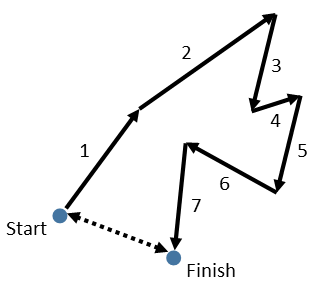
\includegraphics[width=0.5\linewidth]{../images/random-walk}
		\caption{Random walk of a particle with varying step sizes and directions. For an unbiased walk, the displacement from start is expected to be zero.}
		\label{fig:random-walk}
	\end{figure}
	
	Observing the solution from a macroscopic level, it appears that these collisions result in the movement of particles from an area of high concentration to an area of low concentration. The process is observable until the system has reached a particle concentration equilibrium. This equilibrium is a dynamic state, not a static one; overall diffusion may have stopped, but particles continue to move.	Even with the introduction of semi-permeable boundaries separating a high particle concentration region from a low concentration region, if the particle is able to permeate the boundary, an equilibrium can still occur because particle flux across the boundary is equal in opposite directions.
	
	In the simple cell models developed and analyzed, the region in which particles may exist is heterogeneous since it is divided by semi-permeable boundaries and each boundary encloses a region of different diffusivity. The diffusion process still occurs, but particle motion is mediated by the absolute reflecting boundaries of the system and more importantly, by the semi-permeable boundaries. The semi-permeable boundaries behave in a passive transport manner and are considered to facilitate the process of simple diffusion. The boundary conditions necessary to simulate passive transport and required to reach an equal concentration equilibrium are explained later in ``Detailed Balance".
	
	In order to perform an analysis of diffusion behaviour in the simple cell models, a measure for the extent of particle motion was necessary. In the case of undirected motion, the time-average particle position $ \langle x \rangle $ is not a very useful quantity. Although the particle moves randomly, the expectation value for the position is equal to its starting position $ x_0 $. The time-average position-squared $ \langle \Delta x^2 \rangle $, also known as the mean-squared-displacement (MSD), is not equal to $ x_0 $. The MSD may be computed if individual particle positions are known or if the particle density distribution is known at some time $ t_n $. Let $ x_i $ be the position of the $ \textrm{i}^\textrm{th} $ particle at $ t_n $, the MSD is:
		
	\begin{equation}
		\langle \Delta x^2 \rangle = \langle x_{i}^2 \rangle + \langle x_i \rangle^2
	\end{equation}
	
	The MSD calculated at each time step can be used to derive other quantities of interest such as the effective diffusivity constant $ D_\textrm{eff} $ at any point in time. Albert Einstein related the macroscopic diffusivity constant to the microscopic random walk via the MSD \citep{diffusion-1}.
	
	\begin{equation}
	\label{eq:einstein-diffusion-steady}
		\langle \Delta x^2 \rangle = 2Dt \cdot d
	\end{equation}
		
	Where $ D $ is the diffusion coefficient and $ d $ is the dimensionality of the system ($ d = 1 $ was used for all calculations since we were interested only in the MSD in one direction). Solving for the effective diffusivity:
	
	\begin{equation}
		D_\textrm{eff} = \dfrac{\langle \Delta x^2 \rangle}{2t}
	\end{equation}	
	
	Einstein's diffusion equation as we may call it, says that the MSD scales linearly in time. While this is true for \textsl{steady diffusion}, this is not always true for systems where \textsl{anomalous diffusion} occurs. For a system undergoing a steady diffusion process, the log-log plot of MSD versus time has a slope of unity, since $ t $ is raised to the power of 1 in Equation \ref{eq:einstein-diffusion-steady}. For most systems studied, there was some non-linearity in time indicating the presence of anomalous diffusion. 
		
	\begin{figure}[h]
		\centering
		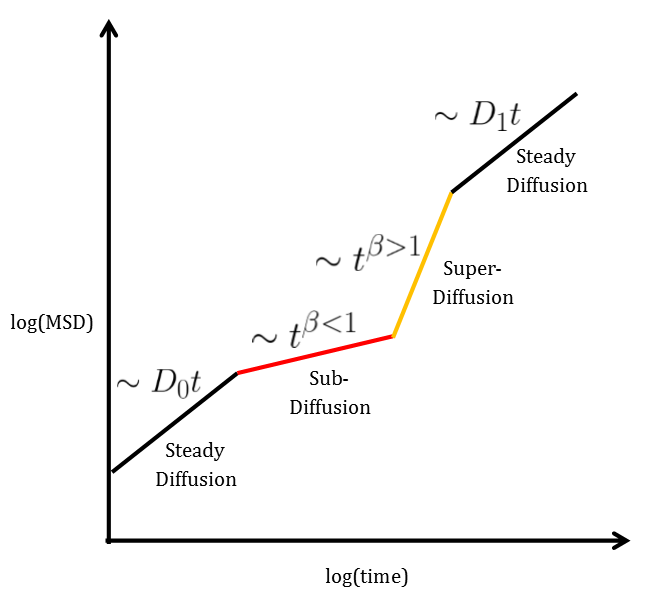
\includegraphics[width=0.7\linewidth]{../images/diffusion-regime}
		\caption{Three diffusion behaviours are observed in the simple cell models.}
		\label{fig:diffusion-regime}
	\end{figure}

	
	We introduce a modified Einstein's diffusion equation with an additional exponential factor $ \beta $, to calculate a quantity $ \beta (t) $ that is useful for characterizing the kind and magnitude of the anomalous diffusion process at any time.
	
	\begin{equation}
	\label{eq:einstein-modified}
		\langle \Delta x^2 \rangle = 2D \cdot t^{\beta}
	\end{equation}
	
	Taking the base-10 logarithm of both sides of Equation \ref{eq:einstein-modified}:

	\begin{equation}
		\log\left( \langle \Delta x^2 \rangle \right) = \beta \cdot \log(t) + \log(2D)
	\end{equation}	
	
	On a linear plot, this appears as a relation of the form $ Y = \beta X + C $ and if $ \beta = 1 $, then the diffusion process is steady. It is possible to determine what $ \beta $ is as a function of time. If we take the derivative $ dY/dX $, then:
	
	\begin{equation}
		\dfrac{dY}{dX} = \beta (t)
	\end{equation}
	
	A plot of $ \beta (t) $ versus $ t $ reveals the magnitude of the non-linearity and identifies if the diffusion process occurring sub- or super-diffusive at a particular time. For a sub-diffusive process $ \beta < 1 $, for a super-diffusive process $ \beta > 1 $, and for steady diffusion $ \beta = 1 $.
	
	\begin{equation}
		D_\textrm{eff} = \dfrac{\langle \Delta x^2 \rangle}{2t}
	\end{equation}
	
	Plots of $ D_\textrm{eff} $ and $ \beta $ versus $ \log (t) $ may be constructed and are useful in determining how the long-time effective diffusivity depends on the semi-permeable boundary transition probability, ratio of cellular to extracellular diffusivities, and system geometry.
	
\subsubsection{Detailed Balance}

	An expected result of all simulations was that the long time particle density distribution is equal across all space. In order for that to occur, special consideration was needed for the semi-permeable boundaries so that the simulations produced the correct results. Consider a very simple system; two regions $ A $ and $ B $ of different diffusivities are separated by a semi-permeable boundary (Figure \ref{fig:balance}). On the left of the boundary at some point $ j $ there is a particle density $ \rho_j $. On the right of the boundary at $ j+1 $ there is a particle density $ \rho_{j+1} $. 
	
	\begin{figure}[h]
		\centering
		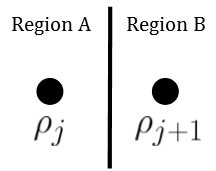
\includegraphics[width=0.27\linewidth]{../images/balance}
		\caption{}
		\label{fig:balance}
	\end{figure}
 
	
%	An argument can be made that, in the higher diffusivity region, particles interact with this boundary more frequently than in the lower diffusivity region.

	Detailed balance theory is useful in understanding and creating boundary conditions to correctly model the dynamics of this two-state system. If the probability of a transition from some state $ A $ to state $ B $ is $ P(A \rightarrow B) $ and the reverse, $ P(B \rightarrow A) $, are known, then it is possible to determine what the equilibrium condition is for the particle densities. That condition is:
	
	\begin{equation}
		\rho_{j} \cdot P(A \rightarrow B) = \rho_{j+1} \cdot P(B \rightarrow A)
	\end{equation}
	
	For our simulations, the total transition probability of a particle to cross a boundary is the product of two independent probabilities; the probability to step towards that boundary $ P_{i \: \textrm{or} \: e} $ and the probability that the particle is successful in transitioning that boundary $ P_{i \rightarrow e \: \textrm{or} \: e \rightarrow i} $ (since the two events are considered mutually exclusive) \citep{haan}. Therefore, in our simulations:
	
	\begin{equation}
		\rho_{j} \cdot P_{i} \cdot P_{i \rightarrow e} = \rho_{j+1} \cdot P_{e} \cdot P_{e \rightarrow i}
	\end{equation}
	
	In the long time, if the condition that particle density is at uniform equilibrium, then  $\rho_{j} = \rho_{j+1} $. Therefore:
	
	\begin{equation}
		P_{i} \cdot P_{i \rightarrow e} = P_{e} \cdot P_{e \rightarrow i}
	\end{equation}
	
	This relation shows what we refer to as coupled boundary conditions. Setting the transition probability $ P_{i \rightarrow e} $ to some value automatically specifies $ P_{e \rightarrow i} $.

\subsubsection{Time and Length Scales}

	From the Einstein diffusion equation, it is possible to map between simulation time and length and physical time and length. This was not done since there was no time left to work on this.

\clearpage
\section{Monte Carlo Theory}
\label{sec:intro-mc}
	
	The term ``Monte Carlo" (MC) summarizes a large number of methods; with some methods simple and others more complex. However, all of the MC methods are based on the sampling of random numbers. In general, MC methods offer the advantage of computational strength, particularly in cases where it is simply not feasible to employ deterministic methods. For our purposes, the motivation to use MC was the nature of the diffusion process, at least at a microscopic level, and the fact that particle trajectories (position history) can be maintained for each particle. This method of simulating diffusion is a particle-based approach to diffusion.
	
	The MC method utilized in our simulations is a basic method and can be referred to as lattice-MC (LMC).  What follows is a overview of the process. At each time step, a pseudo-random number is drawn from a uniform distribution\footnote{Random number generation is a scientific field in itself. It is difficult to generate a purely random sequence of numbers and the distribution sampled was probably approximately uniform. These limitations were likely not of great importance in our simulations.}. This random number is then tested for membership within intervals defined by probabilities and based on the interval the random number is a member of, a specific action is taken.
	
	\begin{figure}[h]
		\centering
		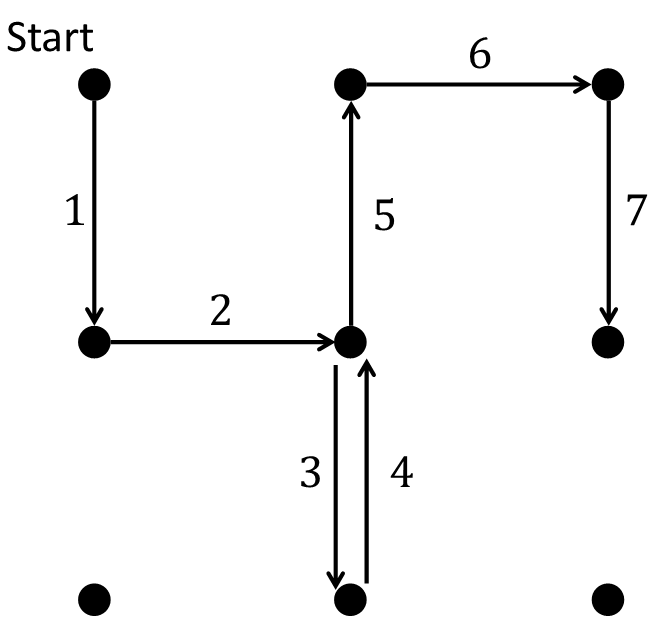
\includegraphics[width=0.5\linewidth]{../images/mc-random-walk}
		\caption{Monte Carlo random walk on a 2D lattice. In our simulations, the step-sizes were fixed length and only on directional step was allowed each time step.}
		\label{fig:mc-random-walk}
	\end{figure}

	This basic method is best described with an example. Consider a 1D system where the diffusivity is $ D = 0.2 $. The probability of a particle to step in a direction is $ P = 0.2 $ (this is true for our simulations and can be shown). We define a set of intervals: $ (0,0.2] $, $ (0.2,0.4] $, and $ (0.4,1.0] $, and with each interval assign an action. If the random number $ rnd \in (0,0.2] $, then the particle moves left. If $ rnd \in (0.2,0.4] $, then the particle moves right. If the number generated is not in those intervals, then for the next time step the particle stays at its current lattice site.
	
	`Moving' the particles is quite simple, if the region is simple and there are no boundaries. Attention must be paid to the position of the particle so that the correct probabilities of stepping in the various directions are applied.
	
	

\clearpage
\section{Master Equation Theory}
\label{sec:intro-me}
	With an enormous number of particles, all randomness disappears and it looks as though the particles move smoothly and deterministically from areas of high concentration to low concentration.
	
	\begin{figure}[h]
		\centering
		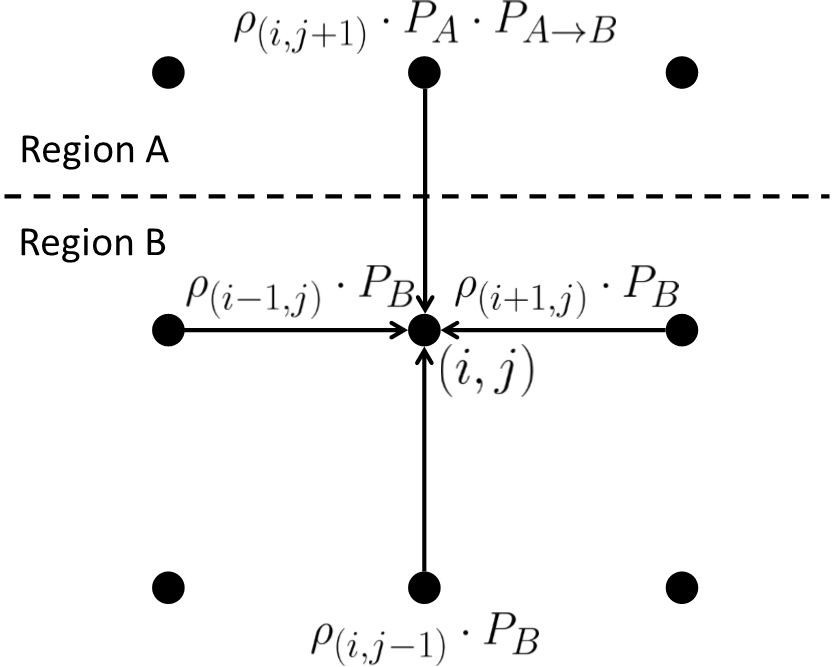
\includegraphics[width=0.6\linewidth]{../images/fd-distribution}
		\caption{Distribution approach on a lattice for diffusion in 2D. Each density and probability product represents the `amount' of density. Not shown is the particle density that `stays' at $ (i,j) $, $ \rho_{(i,j) \cdot P_S} $ where $ P_S $ is the probability that particles stay at the current lattice site.}
		\label{fig:fd-distribution}
	\end{figure}

\clearpage
\section{Simple Cells and Tissues}
\label{sec:intro-cells}
	Nearly all human cells are microscopic in size; their diameters range from 7.5 \si{\micro\meter} to approximately 150 \si{\micro\meter} and a cell exhibits a particular size or shape that reflects the specific task it's designated to perform. There are many different types of cells including nerve cells, muscle cells, and gland cells, but despite their anatomical and functional differences, the cells of the human body have many similarities. It is a fact that no cell contains all cellular components found in all the cell types, so often a composite cell (Figure {\ref{fig:cellpic_2.png}}) is used to exhibit the most important characteristics. 

	\begin{figure}[h]
		\centering
		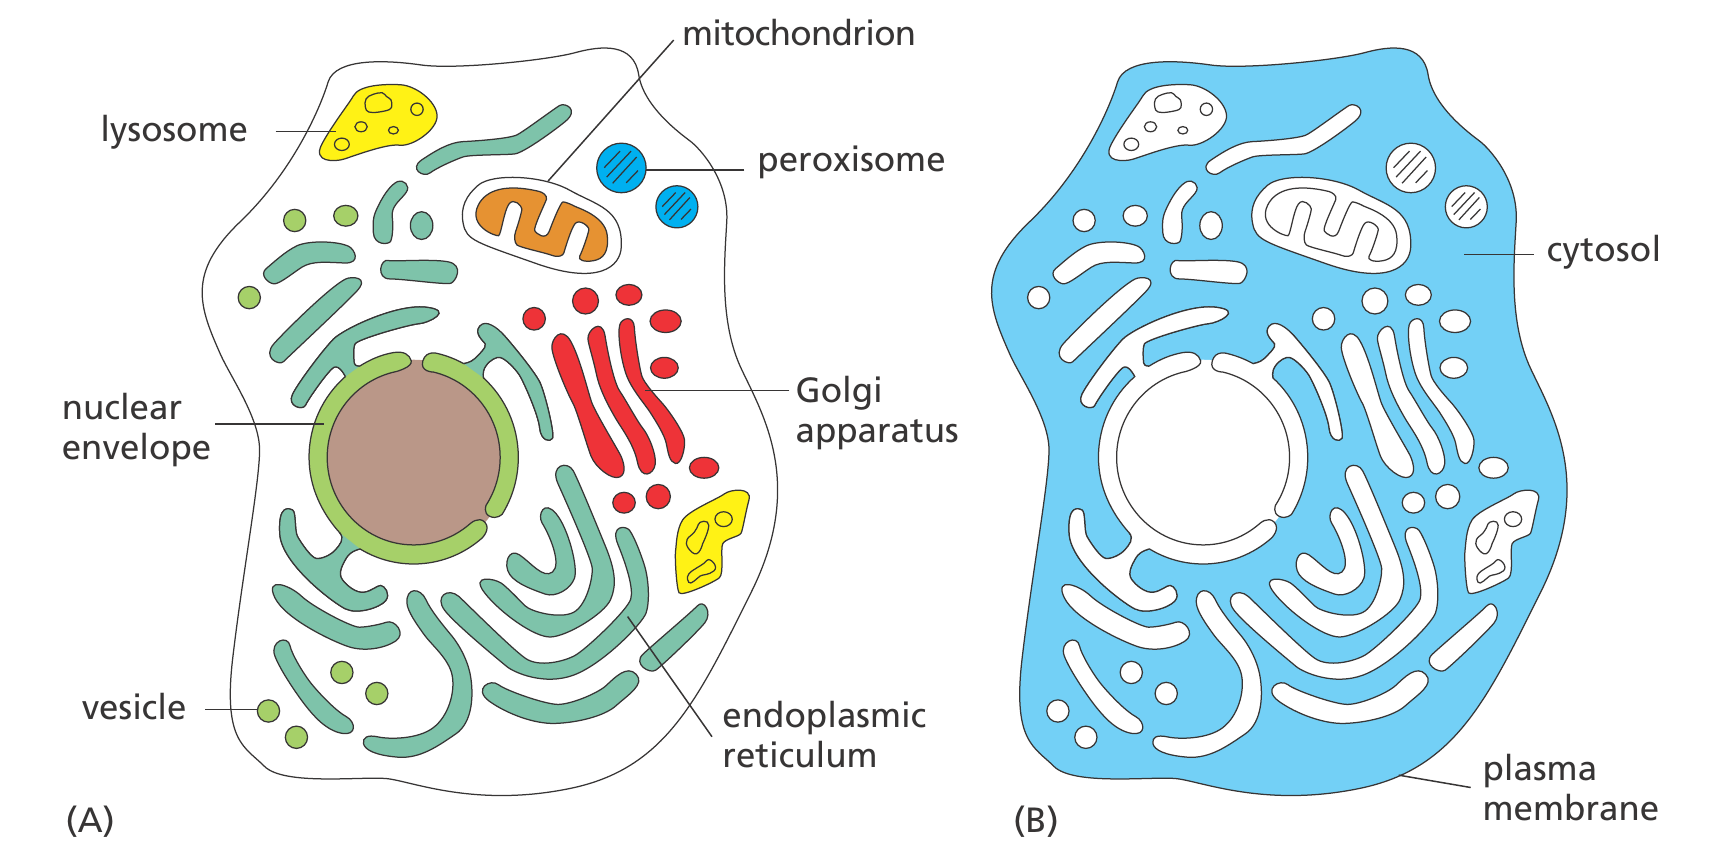
\includegraphics[width=1.0\linewidth]{cellpic_2.png}
		\caption{Composite cell showing various important and common internal cell structures. Most of the volume within the cell is occupied by the cytosol fluid. Figure courtesy of Essential Cell Biology, Alberts, 3rd.}
		\label{fig:cellpic_2.png}
	\end{figure}

	Each cell is enclosed by a plasma membrane that separates the cell contents from the surrounding environment. The inside of the cell is mostly composed of a gel-like substance called cytoplasm that is a dense arrangement of proteins, organelles, and other molecules, suspended in a watery fluid called cytosol. The dense crowding of molecules and organelles results in frequent physical interactions which promotes high metabolic efficiency \citep{ap}. All of the fluid inside the cell may be referred to as intracellular fluid or simply, cellular fluid (CF).
	
	The CF is separated from the extracellular fluid (ECF) by the cell/plasma membrane. This membrane is a phospholipid bilayer with various embedded macromolecular structures. Each phospholipid molecule is amphiphatic, having both a hydrophobic and hydrophilic region. A collection of phospholipid molecules will naturally arrange themselves into a bilayer that does not allow water, polar molecules, or ions to pass through easily. However, water and other molecules or ions need to traverse this membrane and the water transporting task is accomplished by aquaporin gated channel proteins. Aquaporins facilitate the passive diffusion of water through the plasma membrane, between the intracellular and extracellular regions. \citep{ap}.
	
	%These proteins belong to a larger class of proteins called integral membrane bound proteins; some of which act as transporters of various types of molecules or signal transducers.
	
	%Overall, most of the cytosol is water and the viscosity of the cytoplasm is approximately the same as pure water, although the diffusion of small molecules is approximately four times slower than in pure water, due mostly to collisions with the large numbers of macromolecules in the cytosol.

\subsection{Tissues}
	In a multicellular organism, there are several levels of biological organization. A cell is the lowest level of organization that is considered living; tissues are the next higher level of organization and are composed of cells similar in structure and function. This ensemble of cells resides in an extracellular matrix (ECM); a medium containing water, fibrous and adhesive proteins, glycoproteins, and other molecules. The ECM varies in composition between different tissues, but providing structural support and facilitating cell-to-cell communication are common functions of the ECM. In some cells, the cytoplasm is more viscous than the extracellular matrix \citep{cr-biology}. At the cellular level some tissues are relatively organized.
	
	In this project, a simple tissue model was constructed based on some basic defining characteristics of real cells and tissues. The simple tissue model consisted homogeneous spaces, specifically more viscous intracellular regions and less viscous extracellular regions separated by a passive semi-permeable boundary. All of the cells in a model were of the same dimensions and repeated in series.











%Simulation is the imitation of the operation of a real-world process or system over time.[1] The act of simulating something first requires that a model be developed; this model represents the key characteristics or behaviors/functions of the selected physical or abstract system or process. The model represents the system itself, whereas the simulation represents the operation of the system over time.
%
%
%All simulations start with a model. Since the objective of this thesis was to analyze the unbiased diffusion of water molecules in a simple cell or tissue, a model needed to be constructed. It was reasonable to select 
%
%A particular cell or tissue to model is that eukary, any organism that contains . Perhaps the most important defining feature of these eukaryotic cells is that they have membrane-bound organelles and a well defined nucleus. 
%
%First, in order to simulate the diffusion process, a model needed to be constructed. The simple models chosen reflect the basic conditions that might exist in most eukaryotic cells---that is---they contain different compartmental regions separated by semi-permeable membranes.
%
% is intended to imitate of the operation of a real-world process or system over time
%Computers provide an ideal `experimental ground' for simulations that would not be easily feasible or even possible using traditional experimental approaches.
%
%A simple cell model may be used for an approximative analysis of particle diffusion in both 1D and 2D systems.
%
%In the case where the domain of the cell is homogenous (i.e. no internal structures), the calculated effective diffusion coefficient $ D_eff $ is equal to the diffusion coefficient as set in the simulation program parameters. 
%
%As previously mentioned, the goals of this project were to construct a simple-cell model and simulate the process of particle diffusion, under the constraints of absolute boundaries and semi-permeable barriers.
%
%
%
%
%
%
%
%
%
%
%
%
%\section{A sample introduction}
%
%This is just an example, but I wanted to show you some common things to do with Latex.
%
%\subsection{A subsection example}
%
%For of all, here's an equation -- it's the NFW formula, given by \citet{nfw95}, and looks like
%\begin{equation}
%	\label{eq:nfw}
%	\rho(r) = \frac{\rho_s}{r / r_s (1 + r / r_s)^2},
%\end{equation}
%where $\rho_s$ and $r_s$ are a characteristic density and scale radius, respectively.
%
%Now, I can reference that equation later, since it's labelled properly; it's equation (\ref{eq:nfw}).  Notice that I cited a paper above; I could do that in a different way like this \citep{nfw95}.
%
%Just one other quick thing:  figures.  There's one below, and again it's properly labelled.  It's Figure \ref{fig:intro_density}.
%
%\begin{figure}
%\begin{center}
%	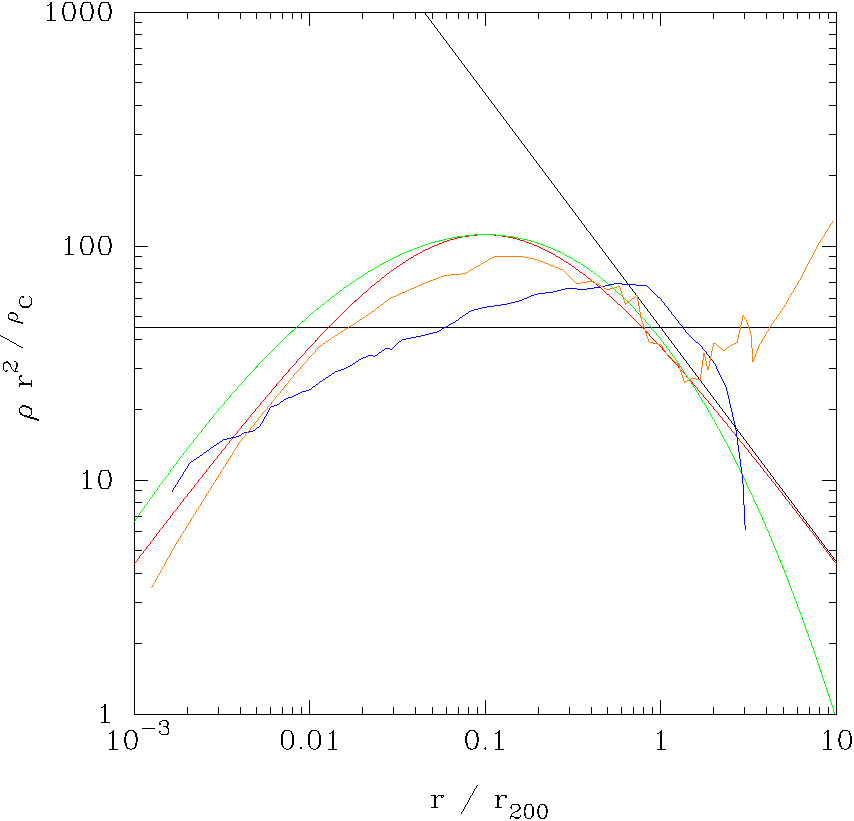
\includegraphics[scale=0.8]{intro_density.pdf}
%\end{center}
%	\caption[Density profiles of various models]{Density profiles, shown as $\rho r^2$ to better highlight the differences, of various models.  }
%	\label{fig:intro_density}
%\end{figure}